\documentclass[UTF8]{ctexart}
\usepackage{graphicx}
\begin{document}
    29,不等价,因为存在方法并没有被返回。

    30,等价,因为所有的调用都完成了,也可以说调用的完成一定实在有穷步完成的。

    32,如下图,A.enq(x)和B.enq(y)分别有其可线性化点,但其第16行代码分别在后边的x,y处执行,这就会使得B.deq(x)的结果是y,结果错误。
    
    \centering
    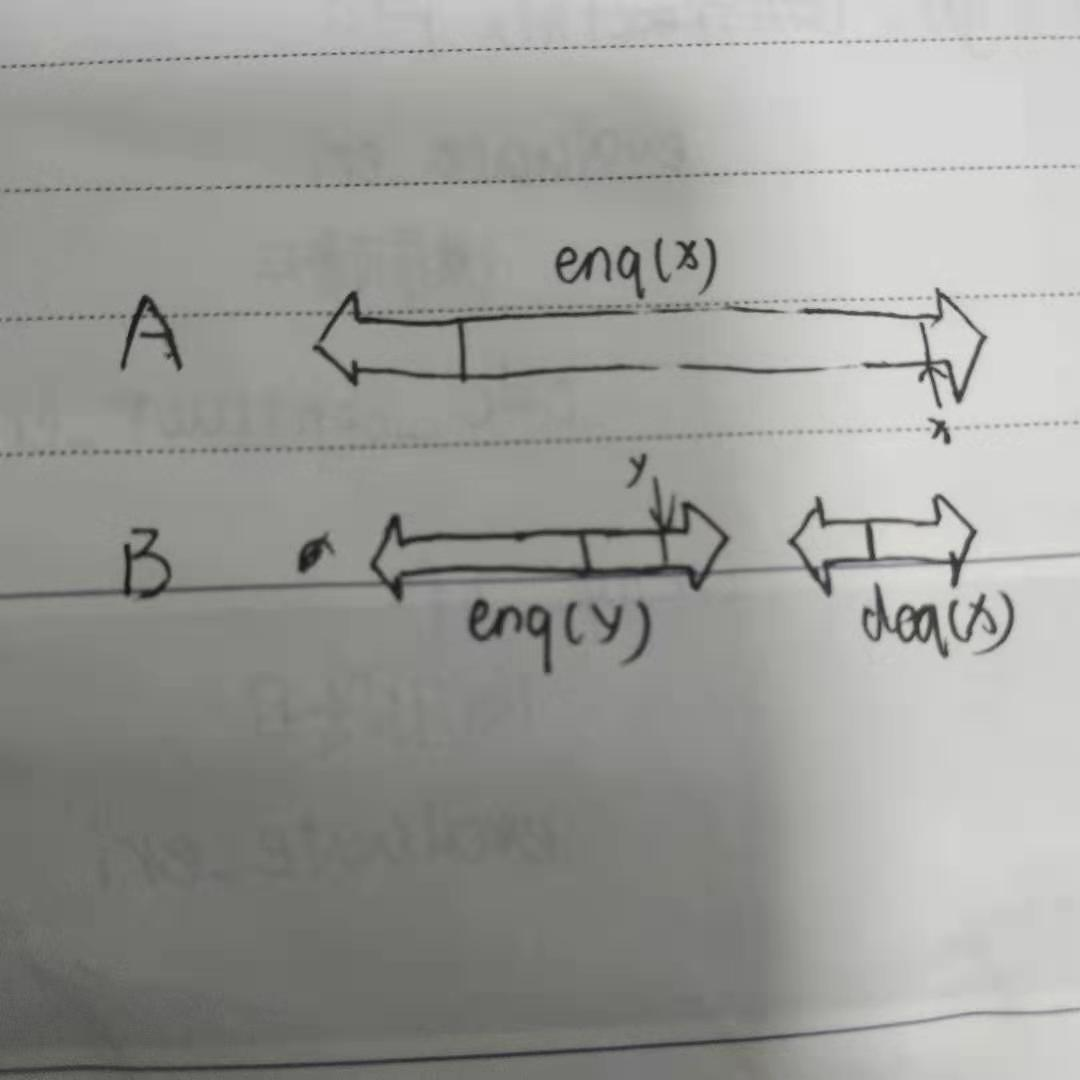
\includegraphics[height=4.0cm,width=7.5cm]{./1.jpg}
    
    如下图,A.enq(x)和B.enq(y)分别有其可线性化点,但其第15行代码分别在后边的x,y处执行,这就会使得B.deq(x)的结果是y,结果错误。
    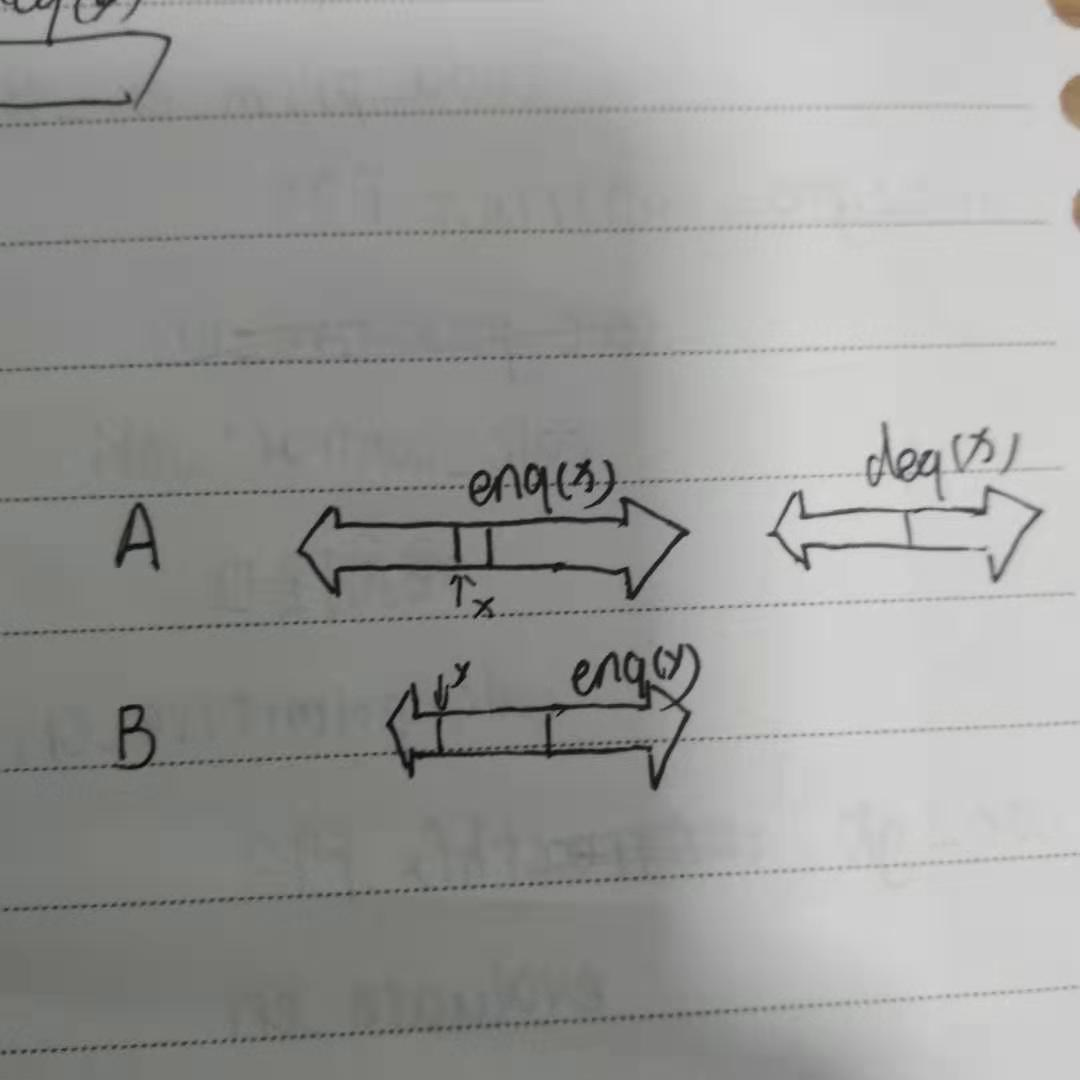
\includegraphics[height=4.0cm,width=7.5cm]{./2.jpg}
    
    33, 因为对一个完全方法的任何未决调用来说,这个调用总是能被完成的。
\end{document}